%
% File: chap01.tex
% Author: Ran Itay
% Description: Introduction chapter.
%
\let\textcircled=\pgftextcircled
\chapter{Introduction}
\label{chap:intro}

\initial{T}he most accredited theoretical framework for the cosmology of our universe, based on numerous cosmological and astronomical observations, is the "$\Lambda$-Cold Dark Matter" model (\cdm). It suggests that only a small fraction ($\sim 5\%$) of the energy density in the universe is in the form of baryonic matter, the rest  $\sim 95\%$ is lurking in the dark~\cite{WMAP:9years, Planck}. The "Dark-sector" consist of \textit{Dark Energy}($\sim 69\%$) and a non-baryonic matter ($\sim 26\%$), \textit{Dark Matter} (DM).

In the 1930s the Swiss astronomer Fritz Zwicky observed that the mass of the cluster inferred by gravitational observation is much larger than the one inferred by the visible luminous light matter. He then deduced the existence of a new type of unseen matter which does not interact with electromagnetic radiation, naming this matter \textit{"dunkle materie"}, \textit{Dark Matter}~\cite{Zwicky:1937zza}. Since then much evidence has been accumulated, suggesting that DM is present at galactic as well as cosmological scales.

In the past decade many experiments joined the hunt for DM detection, and the field has progressed dramatically. These experiments can be divided
roughly into three groups, underground direct detection experiments such as XENON~\cite{xe100_run_combination,Xenon1TResults}, LUX~\cite{LUXnew}, PANDAX~\cite{PANDAX}, CDMS~\cite{CDMSlite}, DAMA/LIBRE~\cite{DAMA} and others , indirect detection in space (FERMI~\cite{FermiLAT:2011ab}, AMS~\cite{AMS}) and on earth (IceCube~\cite{IceCube}), and production experiments in accelerators such as ATLAS~\cite{AtlasDM} and CMS~\cite{CmsDM} at the Large Hadron Collider.
\section{Evidence for the Existence Of Dark Matter}
An extensive amount of observations pointing to the presence of DM at the  single galaxy, inter-galactic and cosmological scales, are present. In this section a brief summary of these observation is presented. 

\subsection{Virial Theorem}

The virial theorem relates the average potential energy density $\left\langle V_p \right\rangle$ of a stationary gravitationally bound system to its mean kinetic energy density $\left\langle T_k \right\rangle $, namely:
\begin{equation}
\left\langle T_k \right\rangle  =-\frac{1}{2}\left\langle V_p \right\rangle.
\end{equation}


In the 1930s Zwicky made the puzzling observation that the velocity dispersion of individual nebulae in the large Coma galaxy cluster contradicts the expectation of the virial theorem, if estimating the total mass solely from the visible matter content~\cite{Zwicky:1937zza}. Additional mass in the form of DM needs to be added to explain the observations. Although Zwicky did not take into account the mass of the hot plasma in the cluster, adding it reduces the discrepancies but doesn't solve it. 

The hot plasma bounded by the gravitational potential of the cluster emits bremsstrahlung X-rays. The x-ray emission is proportional to the plasma density squared. This can be used to estimate the the total mass and mass profile of clusters assuming the cluster is virialized. This type of observations suggest that DM rather than baryonic matter dominates the dynamics of clusters~\cite{Lewis:2002mfa}.

 


\subsection{Galactic Rotation Curves}

The orbital velocity as a function of radius (rotation curve) can be obtained from the measurement of the redshifts of the 1420\,MHz hydrogen transition~\cite{Begeman:1991iy} as well as of spectral lines from stars. The hydrogen cloud extends beyond the galactic disk, allowing the measurement of orbital velocities further out. By measuring the rotation curve of galaxies it is possible to compute their mass profile ($\textrm{M}(r)$).

In 1970 Vera Rubin found a disagreement in the mass profile calculated by the rotation curves and the one expected from luminouse mattter in NGC4605 spiral galaxy~\cite{Rubin:1980zd}. This disagreement can be solved, assuming additional non-visible mass enhancing the gravitational forces.

Formally, assuming Newtonian dynamics
\begin{equation}
\label{v_r}
v(r) = \sqrt{\frac{\mathrm{G}\cdot \mathrm{M}(r)}{r}},
\end{equation} 
where
\begin{equation}
\label{M_r}
\mathrm{M}(r) =  \int_o^r 4\pi \rho(r)r^2dr.
\end{equation}
The majority of a galaxy's luminous mass is situated at the close vicinity of its center  ; therefore if no other mass exist, at large radii one would expect $v(r) \sim r^{-1/2}$. In contradiction the measurements done by Rubin and in many more experiments indicate $v(r) \sim \mathrm{const}$, see Fig~\ref{fig:RotationCurve}. Adding DM with density profile $\rho(r) \sim r^{-2}$ explains this observations.

 \begin{figure}[]
	\centering
	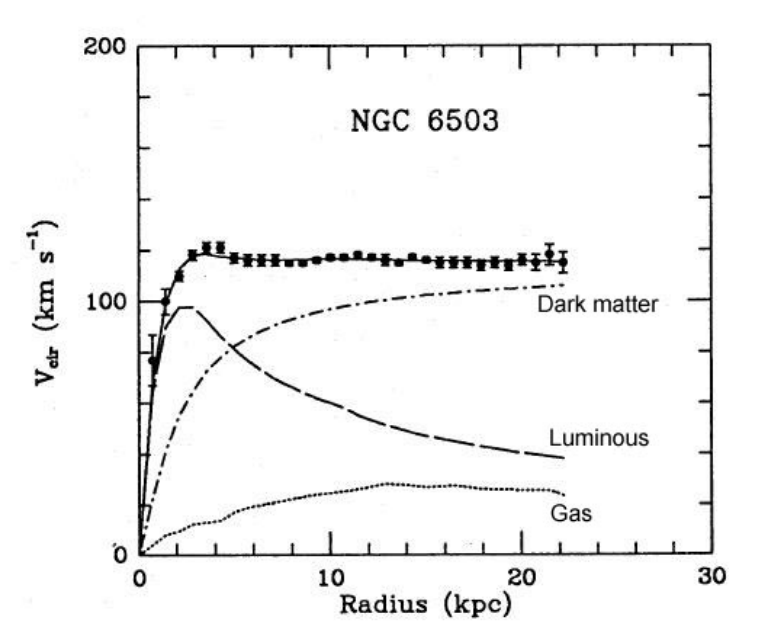
\includegraphics[width=0.8\textwidth]{figs/rotationCurve6503.png}
	\mycaption[Rotation curve of NGC 6503.]{Measured Rotation curve (solid line) of NGC 6503 galaxy. In dashed, luminous component only. In dotted, the gas component, and expected DM halo in dotted-dashed. Image taken from ~\cite{Begeman:1991iy}.}
	\label{fig:emissionType}
\end{figure}  

\subsection{Gravitational Lensing}
  
One of the predictions of general relativity is that trajectory of light in space is determined by the space-time metric, which is determined by the mass distribution. Due to this effect, when a large gravitational potential is located in the line of sight between an observer and a far galaxy, the light from the galaxy is distorted. This phenomena is called Gravitational Lensing~\cite{Bertone:2010zza}. By analyzing the lensed image, the mass profile of the "lens" can be characterized.

\textit{Strong Lensing} is when the gravitational field of the "lens" is so strong it produces multiple images forming an Einstien's cross, as well as Einstein's rings~\cite{Einstein:1956zz}. In Fig.~\ref{subfig:abell1689} is a picture of the largest lensing galaxy cluster observed, Abell 1689. In Fig.~\ref{subfig:QSO} is the a lensed, multiple image picture of the quasar QSO-2237. 

\begin{figure}
   \centering
    \begin{minipage}[c]{0.38\textwidth}
    \centering
    \subbottom[]{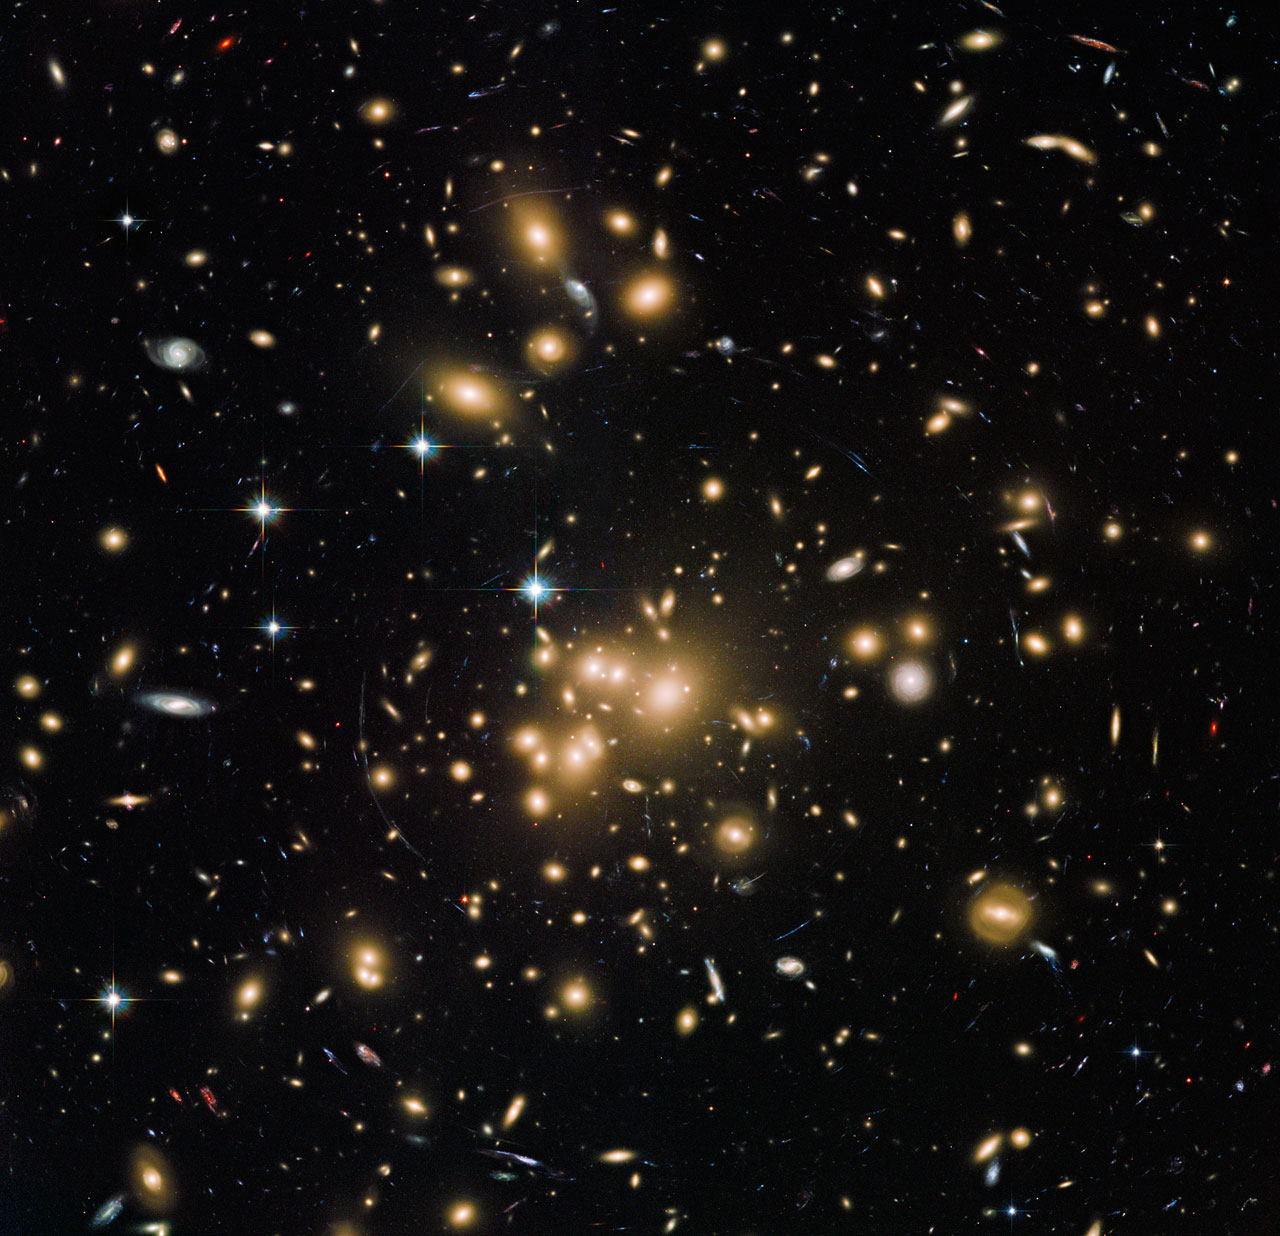
\includegraphics[width=\textwidth]{figs/hubel1689.jpg}
%        \caption{The cryostat and the collimator shining just some of the FV }
        \label{subfig:abell1689}}
    \end{minipage}
    \begin{minipage}[c]{0.4\textheight}%0.49\textwidth , 0.9\textheight}
	\centering    
        \subbottom[]{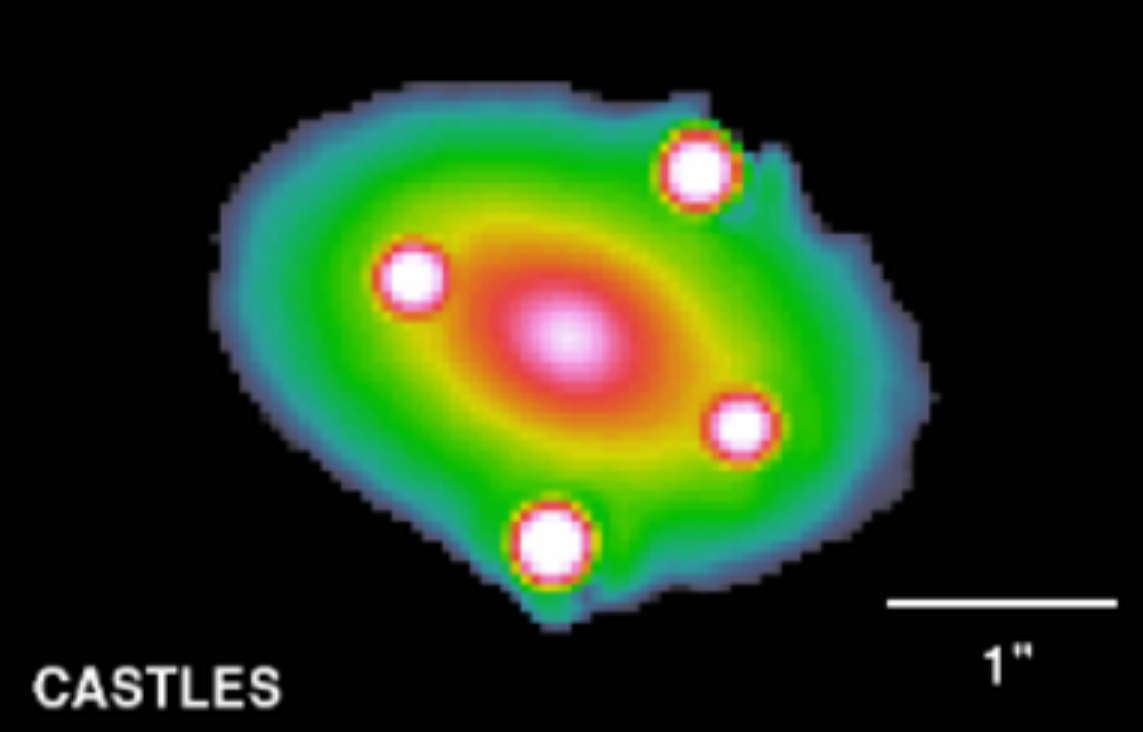
\includegraphics[width=\textwidth]{figs/QSO.png}
%        \caption{a CAD design of the collimator with the conical hole.}
        \label{subfig:QSO}}
    \end{minipage} 
    \caption{ (a) Hubble Space Telescope Advanced Camera for Surveys image of the lensing cluster Abell 1689. Image credit: ESA/Hubble. (b) QSO-2237 quaser lensed image, creating both einstein's arcs and cross. Image credit: CASTLES \label{fig:StrongLens}}
\end{figure}

Two important features are concuded when analyzing the mass profile of the "lens": 1) DM and ordinary matter are not misaligned~\cite{Ferreras:2007na}. 2) The mass profile follows $\rho(r)\propto r^{-2}$ dispersion ratio~\cite{Gavazzi:2007vw}. 

\textit{Weak Lensing} is when the light coming from the source is only weakly distorted by the gravitational lens. In this case it is impossible to detect an individual lensed source; however, multiple background sources align symmetrically around the lens, allowing the detection of the lens mass~\cite{Kaiser:1992ps}.

The most famous weak lensing evidence for DM comes from the "Bullet Cluster", a lensed image of a collision of two galaxies, 1E0657-56 and MACS J0025.4-1222~\cite{Clowe:2006eq}. In this observation (see Fig.~\ref{fig:Bullet}), it is clear that the mass distribution of the luminous and non-luminous matters are spatially displaced. While the luminous matter seems to experienced a violent collision, the non-lominous matter seems to be unaffected. The collisionless behaviour of the DM puts strong constrains on its self inteaction~\cite{Randall:2007ph}. 

 \begin{figure}[]
	\centering
	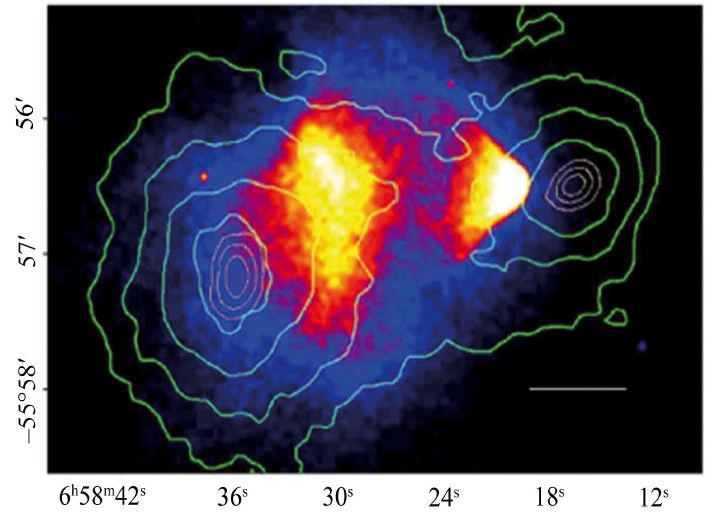
\includegraphics[width=0.8\textwidth]{figs/bulletCluster.jpg}
	\mycaption[Bullet Cluster]{Contours of spatial distribution of mass, from gravitational lensing overplotted over Chandra x-ray data that traces hot plasma in a galaxy. It can be seen that most of the matter resides in a location different from the plasma, which underwent frictional interactions during the merger and slowed down.}
	\label{fig:emissionType}
\end{figure}  



\subsection{Cosmic Microwave Background}
The most precise constraint of the abundance of dark matter in the Universe and a landmark test on the \cdm\ model comes from the measurements of the cosmic microwave background (CMB). The CMB is a reminisce thermal electromagnetic radiation field from the early Universe. 

At the early stages of the Universe, it was hot,dense, and filled with plasma. Then after expanding enough the temperature dropped, and electrons and protons  recombined creating hydrogen atoms. At that stage (reffed as "recombination time"), as the density of free electrons dropped, the thermal radiation could travel freely, without being scattered. These photons propagate through the Universe ever since.       

The CMB follows with extreme precision the spectrum of a black body with temperature of 2.726\,K. It is also known to be very isotropic and temperature  anisotropy is at the scale of $10\mu$K. These temperature fluctuations, considered Gaussian~\cite{WMAP:9years}, are usually expanded using spherical harmonics,
\begin{equation}
\frac{\delta T }{T}(\theta,\phi) = \sum_{l=2}^{\infty}\sum_{m=-l}^{m=l}a_{lm}Y_{lm}(\theta,\phi). 
\end{equation} 

The variance of the coefficient $a_{lm}$ denoted as $c_l$ is defined:
\begin{equation}
c_l \equiv \left< a_{lm} \right> = \frac{1}{2l+1}\sum_{m=-1}^{m=l}a_{lm}^2
\end{equation}

All DM relevance information from CMB can be extracted from the power spectrum of $C_l$ as a function of the multipole $l$. The shape of the power spectrum follows the oscillations of the plasma in the early Universe. In general, the flatness of the Universe can be extracted from the position of the first peak. The ratio between the baryonic and non-baryonic matter is extracted from the ratio between the first 2 peaks.   

More specifically, there are many parameters which affect the CMB spectrum, amongst them are the DM density ($\Omega_{DM}$), the baryonic matter density ($\Omega_{b}$) and the Hubble constant ($h$). Assuming a cosmological model with fixed number of parameters the best fit to the spectrum determines the values of the parameters. The most updated measurment of the CMB spectrum seen in Fig~\ref{fig:CMB} constraine the values of the above mentioned parameters~\cite{Planck} to:
\begin{equation}
\Omega_{DM}h^2 = 0.1197 \pm 0.0022 \qquad \Omega_{b}h^2 = 0.00222 \pm 0.00023 \qquad h=0.67\;[100\, \mathrm{km/s/Mpc}] 
\end{equation}

\begin{figure}[]
	\centering
	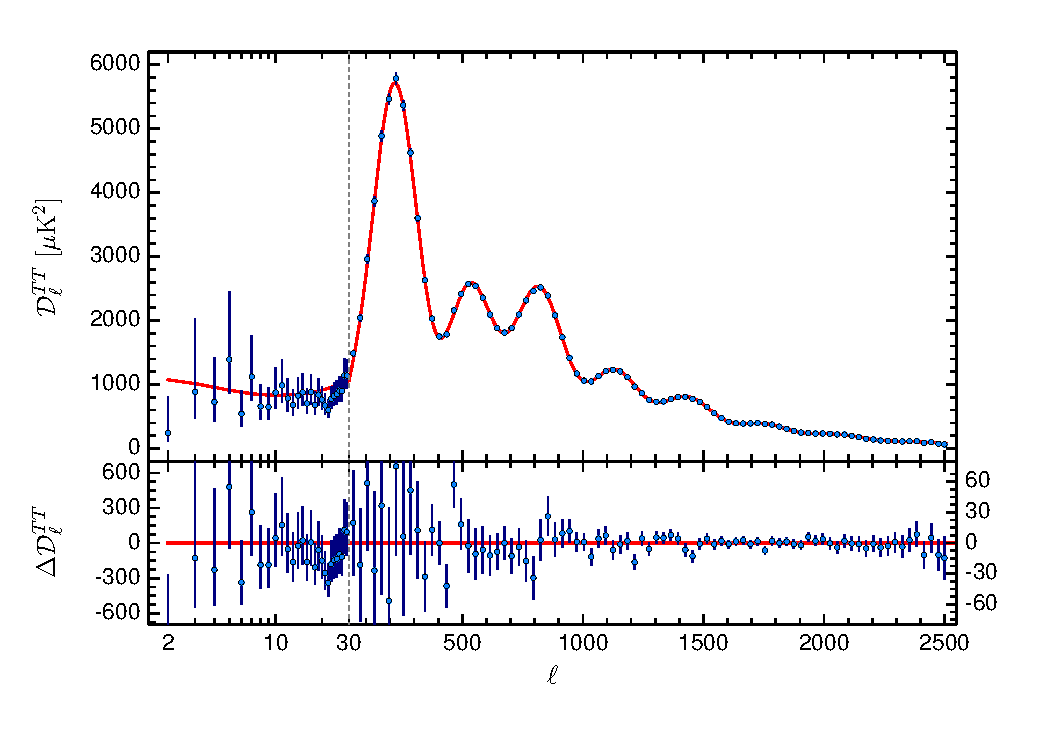
\includegraphics[width=\textwidth]{figs/planck.pdf}
	\mycaption[Plank 2015 CMB power spectrum] {The Planck 2015 temperature power spectrum the solid line is the best fit for the \cdm\ model, the error bars show $\pm \sigma$ uncertainties}
	\label{fig:CMB}
\end{figure}  
  
\subsection{Big Bang Nucleosynthesis}
\label{subsec:BBN}
Big Bang Nucleosynthesis (BBN) is a theory describing the production of the lightest nuclei via a dynamic interplay amongst the four fundamental forces during the first seconds of the Universe~\cite{Jedamzik:2009uy}. The BBN process started when the Universe expanded and became cold enough for electrons and protons to recombine, creating light elements such as Helium, Deuterium, and Lithium, it lasted $\sim20$\,min.

The abundance of the lightest nuclei created in the BBN era can be parametrized by the baryonic density $\Omega_b$ only. This can be done as DM doesn't affect      the expansion rate of the Universe, and the Universe is radiation dominant. The inferred value of $\Omega_b$ which gives the correct abundance, coincide with the one measured by CMB, supporting the existence of non-baryonic matter constituting a large fraction of the matter in the Universe. 
\section{Particle Candidates and Other Solutions to the Dark Matter Problem }
As discussed in previous section there is a large number of convincing evidences for supporting the existence of DM in the Universe, of which its nature is yet unknown. In this section is a short discussion of possible candidates for DM particles, as well as an alternative solution involving the modification of Newton's laws.

\subsection{Axions}

Axions are neutral pseudoscalars initially introduced by Peccei and Quinn in 1977 to solve the "strong CP problem"~\cite{Peccei:1977hh}. The Standard model of particles (SM) contains a CP violating proportional to the parameter $\bar{\theta} = \theta_{weak}+ arg(det(M))$. From measurements  of the electrical dipole moment of the neutron the $\bar{\theta}$ parameter is constrained to be smaller than $10^{-10}$~\cite{Pospelov:2005pr,Baker:2006ts}. The question why the $\bar{\theta}$ parameter is so small is known as the strong CP problem. An elegant solution to this problem is introducing an additional global $U(1)$ symmetry, spontaneously broken producing a Goldstone boson known as the axion. 

Many theoretical and experimental efforts were invested in axion search. The original proposed Peccei-Quinn axion with symmetry breaking scale in the order of the weak scale (246\,GeV) is ruled out; however, axion and axion like particles (ALPs) are still allowed~\cite{Kim:1979if}. For current experimental limits on axions and ALPs see~\cite{Akerib:2017uem} 

\subsection{Primordial Black Holes}
primordial black hole (PBH) are a postulated type of black holes formed at the era before BBN, thus they are not subject to the baryon to photon ration, which gives the baryon density. They were first introduced by Stephen Hawking~\cite{PBH} at 1971, and they can theoretically account for fraction of the DM density~\cite{Carr:2016drx}. 

Limits on the mass of PBH can be placed from the lack
of Hawking-radiated gamma-rays~\cite{MacGibbon:1987my}, combined with null results from microlensing surveys, and constraints based on the CMB~\cite{Ricotti:2007au}. The current allowed mass range of of DM in the form of PBH is ($10^{14}$--$10^{23}$)\,kg.

\subsection{Modified Newtonian Dynamics}
\label{subsec:MOND}

Although the cold dark matter paradigm solves the problems arising from several observations that are mentioned above, there are other paradigms that answer this puzzling observations. The most reasonable is Modified Newtonian Dynamics (MOND)~\cite{Milgrom:1983ca} suggested by Mordechai Milgrom at 1983.

The theory of MOND holds that newton laws should be modified as follows:
\begin{equation}
	f= ma \Rightarrow f= \mu\left(\frac{a}{a_0}\right)ma,
\end{equation}
where $\mu$ is a function between 0 - 1 and $a_o \approx 10^{10}$ is a constant with acceleration units. At high acceleration $\mu =1$ and this reproduces Newton’s law; however at small accelerations $\mu \approx \frac{a}{a_0}$. This small modification solves the mass discrepancies arising from rotation curves up to a factor of 2 which can be easily explained by some baryonic matter that can not be observe because of its weak luminosity.

Although MOND solves the missing mass from rotation curves, in order to solve
the lensing observations one needs to take into account relativistic modifications. The Tensor-Vector-Scalar (TeVeS) gravity~\cite{Bekenstein:2009bd}. Due to the relativistic nature of TeVeS it can explain also gravitational
lensing.

Although MOND and TeVeS can explain some phenomena which are hard to explain in the DM paradigm, They still cannot explain all evidences mentioned above. Mainly observations coming from strong lensing, and CMB still do not have an adequate explanations in these paradigms.


\subsection{Weakly Interacting Massive Particles}
\label{subsec:WIMP}

In order to solve the DM problem it seems natural to extent the matter content in the SM. Ideally a good DM particle candidate, apart from being electromagnetically neutral, should be non-baryonic and stable over the age of the Universe resulting in the correct abundance starting from thermal reactions in the early stage of space and time.

Freeze-out is an appealing mechanism to generate a fixed amount of a specific matter. It is already successfully explained photon decoupling (CMB) and the production of nuclei (BBN). At early stages of the Universe it was hot and dense and particles were in chemical equilibrium between creation and annihilation reactions between various particles and radiation types. DM particles $\chi$ could transform into other SM particles by co-annihilation, or be produced from the same process in SM particles.  
\begin{equation}
\chi\bar{\chi} \Leftrightarrow f\bar{f}, W^+W^-, HH, ...
\end{equation}

The annihilation rate is determined by $R_{ann} = \left<\sigma_{ann}v \right>n$ where $\sigma_{ann}$ is the thermal average of the self-interaction cross section, $v$ and $n$ are the relative velocity and number density of DM particles respectively. For the creation process, the available kinetic energy of colliding particles must exceed the mass threshold of generating a $\chi\bar{\chi}$ pair. During equilibrium the energy distribution is assumed to be thermalized and follow a Maxwell-Boltzmann distribution $e^{E/K_BT}$. When the Universe expanded enough, the temperature dropped and collision of SM particles were not energetic enough the create DM $\chi\bar{\chi}$ pairs, causing the number density of DM to decrease faster then SM particles. At some point the Universe expansion rate became larger than DM annihilation rate causing the number density of DM to freeze-out. 

%TODO Im here

%This
%moment defines the persisting particle number inside a comoving volume. The evolution is illustrated
%in Fig. 1.5, where the number density is drawn as a function of 1{T, proportional to the time passed
%after perfect equilibrium. From the detailed calculation of the abundance evolution, the freeze out
%temperature (in units of energy or mass) is expected around T f  mχ{20, as 
\begin{figure}[]
	\centering
	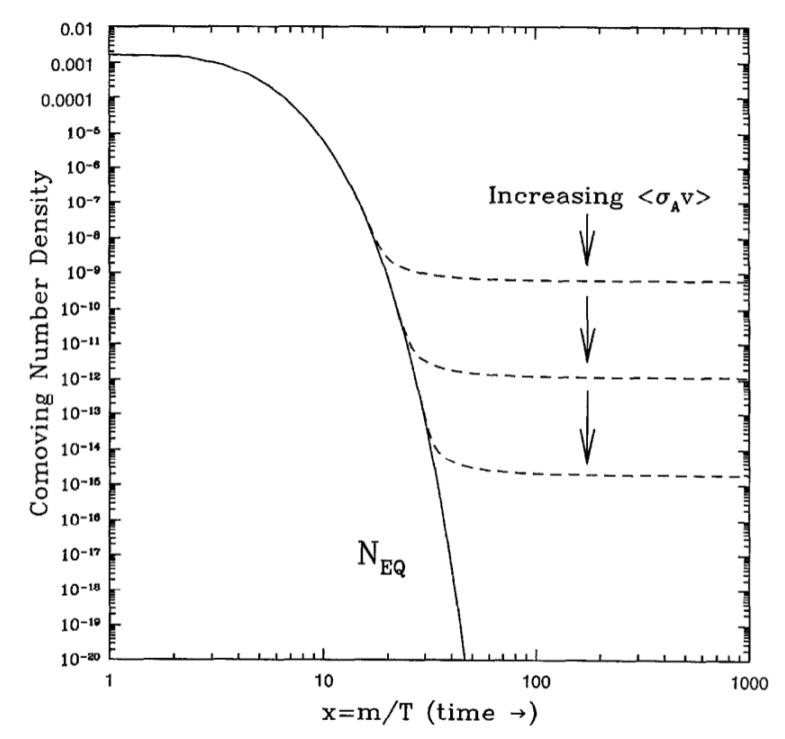
\includegraphics[width=0.6\textwidth]{figs/WIMP_Miracle.jpg}
	\mycaption[WIMP freeze out] {Evolution of the dark matter number density 		as a function of mass over temperature in the universe (proportional to increasing time after the Big Bang). Different assumed annihilation cross-sections $\sigma_{ann}$ lead to differing relic dark matter number densities. Image taken from~\cite{Jungman:1995df}}
	\label{fig:CMB}
\end{figure}  

%%======
\section{Non Linear Emission of Radiation in Liquid Xenon}
\label{sec:intro_superradiance}
As explained in (~\ref{} TODO add reference here) in LXe based experiment the exact properties of the scintillation and ionization responses to all types of interaction must be well quantified and understood. Mainly, much research has been focused on the scintilation and ionization responses of LXe to events with energy recoil as low as <O(10\,keV)~\cite{Manzur:2009hp,Aprile:2012an,Baudis:2013cca}(TODO add LUX).
Specifically the reconstruction of the directionality of recoil nuclei or electrons is of great interest to DM direct detection experiments. Better understanding of these properties may help to reduce background dramatically.

Several existing and proposed experiments such as DRIFT-II~\cite{Muna:2007zz}, DMTPC~\cite{Deaconu:2017vam}, NEWAGE~\cite{Yakabe:2016pjh} and MIMAC~\cite{Riffard:2016mgw}, exploit recoil direction properties. However These experiments are using dilute gas in which the ionization tracks extend to a few millimeters. However, in LXe the track length is estimated to be O(100nm). Moreover the topology of the excimers clouds is represented by a complex structure of branches which are formed by secondary recoils [35,50]. These two different properties, track length and structure, makes it highly difficult if not impossible to construct directionality in a LXe experiment. Therefore, a different approach for directionality measurement needs to be adopted for DM LXe based experiments.

The phenomena of an isolated particle in an excited state undergoing a transition to its ground state (i.e. spontaneous decay) as a result of the vacuum electromagnetic field  is well described in the theory of quantum electrodynamics. This theory is applicable for an ensemble of particles only when particles interact with the vacuum electromagnetic field separately. In this case the ensemble will emit light an exponential law. The characteristic time, $\tau_{sp}$, of a single particle to radiate is equal to the the reciprocal of the transition rate $\Gamma$ from the initially excited level. The radiation pattern in this case is isotropic in its nature, see Fig.~\ref{fig:emissionType}a. 

These radiation properties are significantly different when the radiating particles are dense enough. In this case the collective radiation from  the ensemble is different than the sum of all particles radiating. This phenomena was first postulated by Dicke~\cite{DickeSR} in 1954 and was first measured in Xe by Rosenberger in 1965~\cite{FirstMeasure}. In his research the radiation decay time from a two level atomic system was considered and expected to be dependent on the number of radiating particles N. This type of emission is referred as superradiance. This phenomena is due to interaction of the radiating particles with each other via a common electromagnetic radiation field, which results in a correlation between the atomic dipole moment. This correlation leads to a macroscopic optical polarization proportional to N. Hence the radiation intensity is proportional to $N^2$, leading to a pulsed radiation with duration proportional to $1/N$, see Fig~\ref{fig:emissionType}b. The phenomena of superradiance has been studied extensively since see [TODO add cite [52, 53]]   
\begin{figure}[t!]
	\centering
	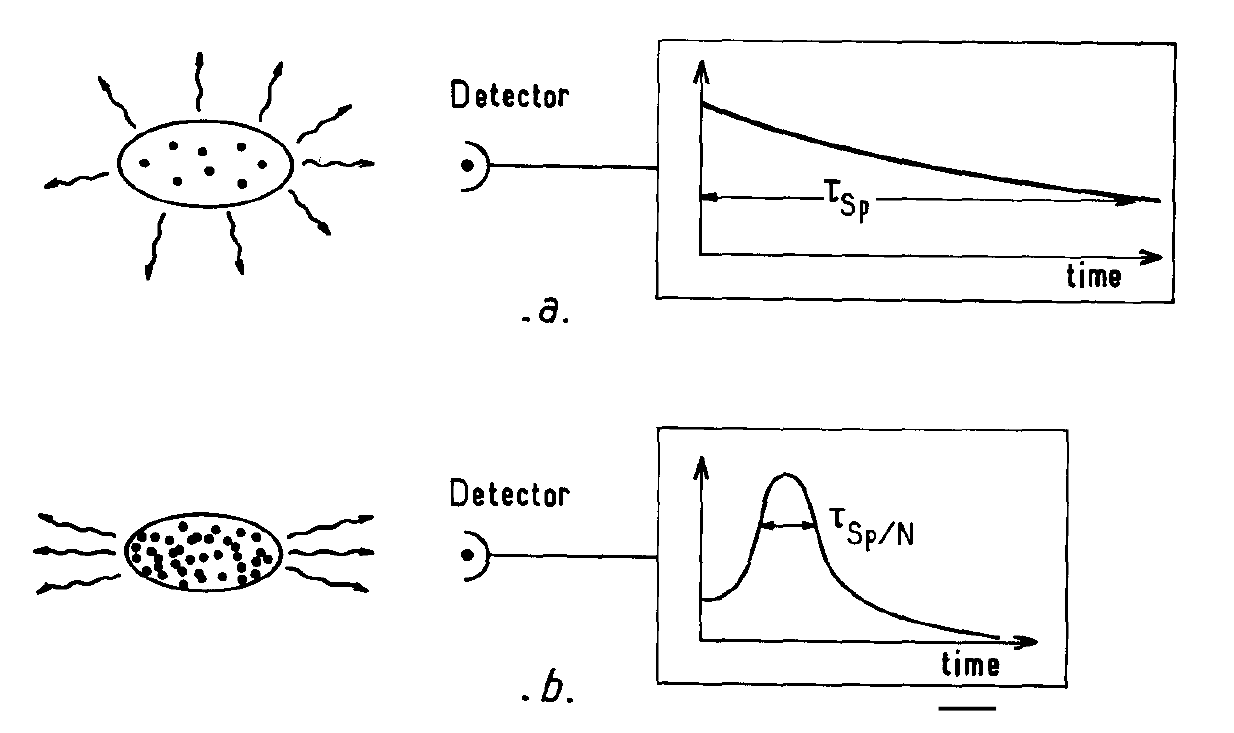
\includegraphics[width=0.8\textwidth]{figs/emissionTypes.png}
	\mycaption[TODO list of figures caption.]{TODO insert caption here}
	\label{fig:emissionType}
\end{figure}


An effective self-induction of correlations between dipole moments is a necessary condition for a particles to exhibit a \superradiance emission. The condition for this to occur are very different then the ones of regular fluorescence. The characteristic time of \superradiance emission to happen, $\tau_c \sim 1/N $ must be shorter the relaxation time of the atomic dipole moment, $\tau_d$. It also has to be shorter then $\tau_{sp}$, however in most cases, $\tau_{d}$ is smaller than $\tau_{sp}$, hence this is a more stiringit condition. Notice that unlike inverse population that happens in lasers, which occurs due to an external "pump", the correlation build-up between the radiating particles in \superradiance happens spontaneously in the course of emission process.

The geometry of the radiating particle ensemble influences greatly weather or not a system will exhibit a \superradiance or standard spontaneous emissions. Specifically the two relevant quantities, are the wavelength $\lambda$ of the emitted photon, and the size of the radiating particles cloud. A system with linear size much smaller then the emitted photons wavelength.   
%The superradiant emission depends strongly on the geometry of the atomic system. The length
%scale relevant for the qualitative behaviour of the emitted radiation is the wavelength , λ, corresponding
%to the atomic de-excitation. If we consider a system of radiators with linear size much
%smaller than λ, i.e. V  λ
%3
%, where V is the volume of the system, the system will emit a pulse in an
%arbitrary direction (isotropic), with an intensity that will reach a maximum Imax ∼ N2
%. However,
%a system with linear size L & λ will radiate most of its energy into small solid angles along the

TODO understand previous paragraph

\section{EFT}
\label{sec:intro_EFT}

The traditional approach for computing predictions of the rate of WIMP-nucleon scattering has been to take only leading-order terms in a WIMP-nucleon effective field theory (EFT) with a very simple treatment of nuclear structure~\cite{LEWIN}. This leads to two main types of interactions, which are commonly labelled ``Spin Independent'' (SI) and ``Spin Dependent'' (SD). However, in recent years many authors have pointed out that in certain theories these interactions may be suppressed or nonexistent, such that otherwise subleading interactions may dominate the scattering process~\cite{Chang:2009yt}. To account for this possibility in a systematic way, a more sophisticated EFT approach has been developed ~\cite{Fitzpatrick:2012ib,Anand:MathTools,Fitzpatrick:MathTools}. In the new approach, an effective Lagrangian describing the WIMP-nucleus interaction is constructed, that takes into account all Galilean-invariant operators up to second order in the momentum exchange. This framework introduces new operators associated with different types of nuclear responses, along with the standard SI and SD ones, resulting in a set of fourteen operators $\mathcal{O}_i$ which may couple independently to protons and neutrons. In Eqs. (\ref{eq:OpDef}) we list these operators following the convention from~\cite{Anand:MathTools}. The operators depend explicitly on 4 linearly independent quantities: $\vec{v}^{\perp} \equiv \vec{v} + \frac{\vec{q}}{2\mu_N} $, the relative perpendicular velocity between the WIMP and the nucleon, $\vec{q}$, the momentum transferred in the scattering event, and $\vec{S}_\chi$, $\vec{S}_N$, the WIMP and nucleon spins. $\mathcal{O}_2$ is not considered here as it cannot be obtained from a relativistic operator at leading order.
%

\begingroup
\belowdisplayskip=0pt
\begin{align*}
\begin{split} 
&\mathcal{O}_1 = 1_{\chi} 1_N  \\
%&\mathcal{O}_2 = (v^{\perp})^2 \\
&\mathcal{O}_3 = i\vec{S}_N\cdot (\frac{\vec{q}}{m_N}\times\vec{v}^\perp) \\
&\mathcal{O}_4 = \vec{S}_{\chi}\cdot \vec{S}_N \\
&\mathcal{O}_5 = i\vec{S}_{\chi}\cdot (\frac{\vec{q}}{m_N}\times\vec{v}^\perp) \\
&\mathcal{O}_6 = (\vec{S}_{\chi} \cdot \frac{\vec{q}}{m_N})(\vec{S}_N \cdot \frac{\vec{q}}{m_N}) \\
&\mathcal{O}_7 = \vec{S}_N \cdot \vec{v}^\perp \\
&\mathcal{O}_8 = \vec{S}_{\chi} \cdot \vec{v}^\perp  \\
\end{split}
\begin{split}
&\mathcal{O}_9 = i\vec{S}_{\chi} \cdot(\vec{S}_N \times \frac{\vec{q}}{m_N}) \\
&\mathcal{O}_{10} = i\vec{S}_N \cdot (\frac{\vec{q}}{m_N}) \\
&\mathcal{O}_{11} = i\vec{S}_{\chi} \cdot (\frac{\vec{q}}{m_N}) \\
&\mathcal{O}_{12} = \vec{S}_\chi \cdot (\vec{S}_N \times \vec{v}^\perp) \\
&\mathcal{O}_{13} = i(\vec{S}\chi \cdot \vec{v}^\perp)(\vec{S}_N \cdot \frac{\vec{q}}{m_N})\\
&\mathcal{O}_{14} = i(\vec{S}_\chi \cdot \frac{\vec{q}}{m_N})(\vec{S}_N \cdot \vec{v}^\perp) \\
\end{split}
\end{align*}
\endgroup
\begingroup
\abovedisplayskip=0pt
\begin{align}
&\mathcal{O}_{15} = -(\vec{S}_\chi \cdot \frac{\vec{q}}{m_N})\left[(\vec{S}_N \times \vec{v}^\perp)\cdot \frac{\vec{q}}{m_N}\right]
\label{eq:OpDef}
\end{align}
\endgroup

Unlike the more commonly studied types of interaction (SI,SD), which are not suppressed when $\vec{q} \rightarrow 0$ and for which the scattering rate on nucleons is expected to be largest for low energy nuclear recoils, some of the new EFT operators depend explicitly on $\vec{q}$ and so their interaction cross section is suppressed for low momentum transfers. Consequently, their scattering rate peaks at non-zero nuclear recoil energy. For sufficiently high WIMP masses, this may even occur outside typical analysis windows, which usually have an upper range of around $ 43\,\keVr$ (nuclear recoil equivalent
energy) since they are designed to search for SI and SD interactions, which predict exponentially-falling recoil spectra (see Figure~\ref{fig:dRdE}). Due to the theoretical bias of only considering SI and SD interactions, high energy nuclear recoils remain unexplored in many experiments.

	    Another typical assumption that can be relaxed is that WIMPs should scatter elastically with nuclei. There exist dark matter models in which the incoming and outgoing WIMPs have different mass states~\cite{InelasticIntro} separated by a keV-scale splitting. In the case where the outgoing state is more massive than the incoming state, the cross section for low recoil energies can again be suppressed, this time by scattering kinematics. Recently an inelastic adaptation of the EFT operator framework discussed above was developed~\cite{InelasticMath}. In this case the operators presented in Eqs.~\ref{eq:OpDef} are modified such that $\vec{v}^\perp_{inelastic} = \vec{v}^\perp_{elastic} +\frac{\delta_m}{\vert{\vec{q}}\vert^2}\vec{q}$. We consider this case in section \ref{subsubsec:Inelastic}.
%\subsection{Subsection}
%\label{subsec:subsec01}
%
%Begins a subsection.
%
%%A figures matrix.
%\begin{figure}[t!]
%\centering
%\begin{minipage}{3.3cm}
%    \centering
%    \subtop[]{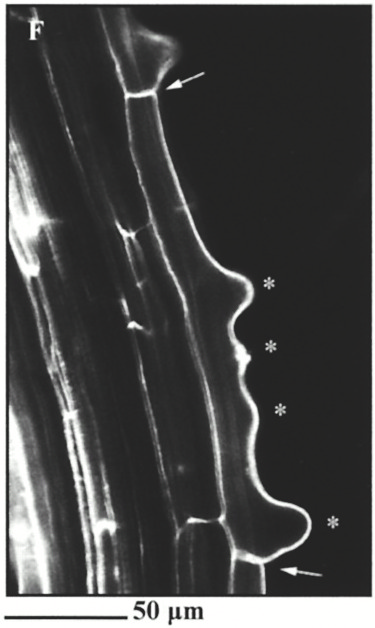
\includegraphics[height=0.28\textheight]{fig01/Nswellings}\label{sf:multiRH02a}}
%\end{minipage}
%\hspace{0.5cm}
%\begin{minipage}{3.3cm}
%    \centering
%    \subtop[]{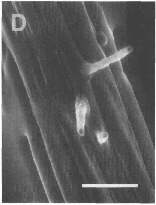
\includegraphics[height=0.27\textheight]{fig01/Mswellings}\label{sf:multiRH02b}}
%\end{minipage}
%\hspace{1.3cm}
%\begin{minipage}{3.3cm}
%    \centering
%    \subtop[]{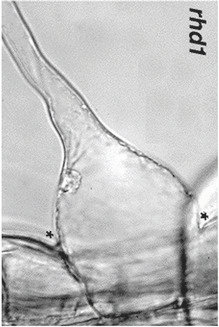
\includegraphics[height=0.27\textheight]{fig01/rhd1}\label{sf:multiRH02c}}
%\end{minipage}
%%\\ \vspace{0.1cm}
%%\begin{minipage}{10cm}
%    \centering
%    \subtop[]{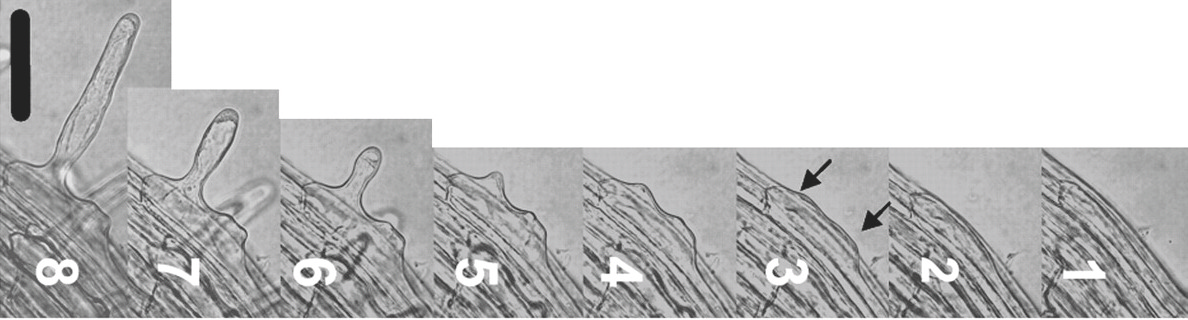
\includegraphics[height=0.145\textheight]{fig01/mutantrhd6}\label{sf:multiRH02d}}
%\end{minipage}
%\\ \vspace{0.1cm}
%\begin{minipage}{10cm}
%    \centering
%    \subtop[]{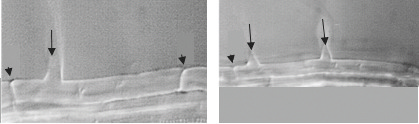
\includegraphics[height=0.16\textheight]{fig01/auxab}\label{sf:multiRH02e}}
%\end{minipage}
%\mycaption[Hair-forming mutant cells.]{(a) A mutant RH cell. Asterisks show multiple sites of RH initiation in a single root hair cell (indicated by the arrows). Figure reproduced from \cite{rigas01}. (b)~Hair-forming cell with three RH initiation locations. The bar represents $50\mu m$. Figure reproduced from \cite{massuci01}. (c) Large bump in mutant {\itshape rhd1}. Figure reproduced from \cite{griersonRH}. (d) Mutant overexpressing gene {\itshape ROP2}; from right-hand to left-hand, numbers indicate progressive snapshots at different times. RH initiation sites are indicated by the arrows. The bar represents $75\mu m$. Figure reproduced from~\cite{mjones01}. (e)~Mutants affected by auxin. On the left-hand side, RH site is farther away from the apical end (left arrow cap); on the right-hand side, multiple RH locations (arrows). Figure reproduced from~\cite{payne01}.}
%\label{fig:multiRH02}
%\end{figure}
%
%% A single figure
%\begin{figure}[t!]
%	\centering
%	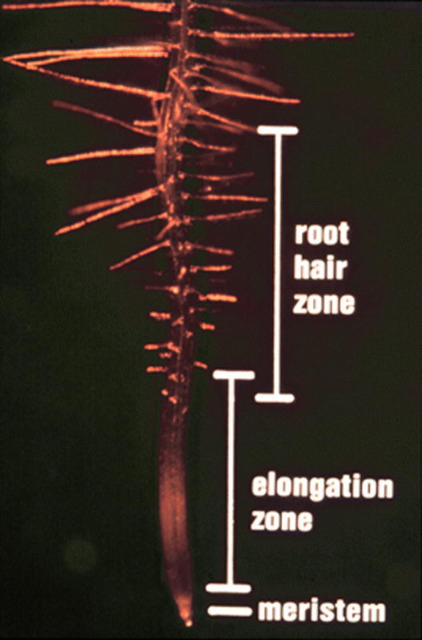
\includegraphics[height=0.35\textheight]{fig01/devepzones}
%	\mycaption[Developmental zones of an Arabidopsis root.]{Developmental zones of an Arabidopsis root. Figure reproduced from \cite{griersonRH}.}
%	\label{fig:RHP02}
%\end{figure}

%=========================================================